\section*{HSL: Experimentación}

Al igual que en los anteriores filtros, esperabamos que el rendimiento de nuestra implementación en assembler sea más rápida que la de C. Sin embargo los resultados nos dijeron lo contrario.


\begin{figure}[!hbt] 
	\centering
  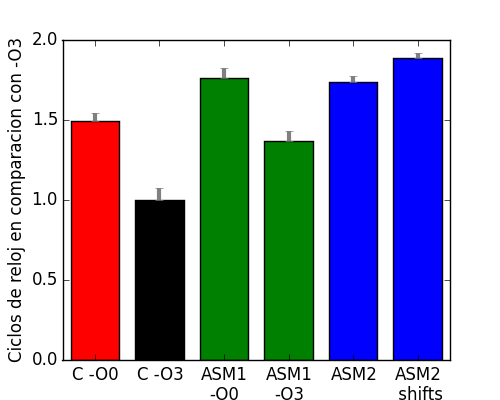
\includegraphics[width=10cm]{hsl.png}
  \caption{Comparación de la cantidad de ciclos de reloj utilizada por diferentes variantes de hsl. Para tener una medida absoluta: la cantidad de ciclos de reloj promedio de C -O3 es 31,620,627. Tamaño de la muestra: 200 imagenes de $16 \times 10^4$ píxeles. Se indica el mínimo con la barra y el promedio con una linea gris.}
\end{figure}

Los resultados fueron devastadores, dado que no los esperabamos. Al igual que el resto de los filtros, el comportamiento de los algoritmos es lineal sobre la cantidad de píxeles, pero la pendiente de nuestras implementaciones de assembler es mayor que las de C.

Por esta razón nos propusimos a hacer un amplio análisis de la situación, para poder descubrir la razón del bajo rendimiento.

La principal limitación de nuestra implementación de assembler son, claramente, los accesos a memoria. En cada rutina (de ambas implementaciones) debemos cargar muchas constantes que usaremos a lo largo de las distintas cuentas que debemos hacer.
Esto es muy caro para nosotros, dado que los accesos a memoria son de lo mas limitante en lo que concierne a la performance. 
A esto atribuimos principalmente nuestro pobre desempeño frente a la implementación de C. Veremos más adelante otras circunstancias que apoyan esta teoría.

Habiendo dicho esto, también es cierto que una vez que pedimos un dato de memoria, este debería guardarse en la cache, siendo su acceso mucho más rápido. Pero la cache sigue siendo aún mas lenta que los registros del procesador, por lo que acceder a memoria (por mas que sea cache) sigue siendo un factor limitante.
\\

Al ver los resultados, nos propusimos cambiar la implementación de assembler. Nuestra primera versión utilizaba muchos shifts, y dado que en una clase vimos que el desempeño de los shifts era peor que el desempeño de los shuffles, decidimos probarlo. El resultado, como se ve en la primera imagen, no fue del todo el esperado. Sí, hubo una mejora de performance, pero no fue significativa, ni nos permitió acercarnos a la implementacion en C, nuestro principal objetivo.


\begin{figure}[!hbt] 
	\centering
  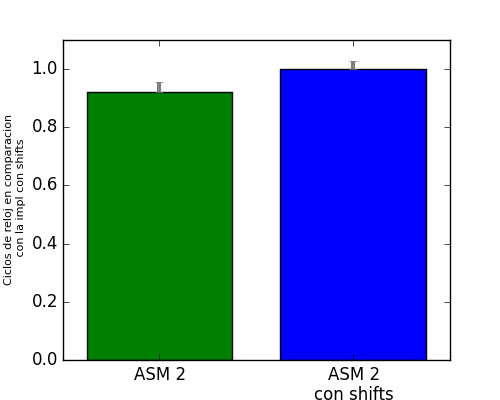
\includegraphics[width=10cm]{hsl-shsh.png}
  \caption{Comparación de la cantidad de ciclos de reloj utilizada por dos variantes de hsl2. Tamaño de la muestra: 200 imagenes de $16 \times 10^4$ píxeles. Se indica el mínimo con la barra y el promedio con una linea gris.}
\end{figure}

Como se ve en esta imagen claramente, este cambio solo nos permitió un magro 10\% de ganancia sobre la implementacion de C.

Algo importante que notar es que esto no significa que usar shuffles es 10\% más rápido que usar shifts, si no que es bastante más rápido. Esto se debe a que nostros hacemos el análisis del programa completo, si se analizan por separado las partes en las que esta decisión incumbe, se llega a speedups de hasta el 40\%, dependiendo de la computadora.
\\

Por otro lado, nuestros algoritmos no dependen fuertemente en saltos condicionales, usan los necesarios, por lo tanto no creemos que este sea un factor limitante del rendimiento.
\\

La siguiente limitación de nuestra implementación es la operatoria de las conversiones de RGB a HSL y viceversa. Esto se debe a que las operaciones que se deben hacer son largas y costosas, por mas que esten lo mejor optimizadas posibles.

A esto se le suma la dificultad de operar de a muchos píxeles juntos, dado que solo se puede en pequeñas partes.
Por ejemplo, en hslTOrgb se podría calcular de forma paralela c, x, m para 4 pixeles así como la operatoria de los shuffles.
Sin embargo, la complejidad del código crece enormemente, sumado a que la operación de rgbTOhsl y la de Suma no son así de simples de paralelizar.
Por estas razones, optamos por no probar esta variante del código, pero es una opción a tener encuenta
\\

Comentando partes de códigos, pudimos obtener una partición tentativa de cuanto tarda cada operacion de la segunda implementación de hsl, algo que nos parece vital a la hora de analizar la performance. Los resultados fueron los siguientes:


\begin{figure}[!hbt] 
	\centering
  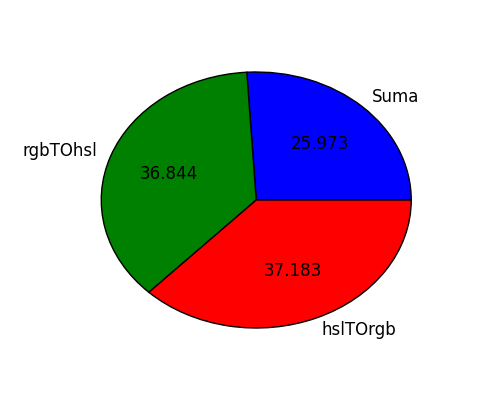
\includegraphics[width=10cm]{hsl-div.png}
  \caption{Análisis comparativo del porcentaje de tiempo dedicado a cada instancia. Tamaño de la muestra: 100 imágenes de $16\times 10^4$ píxeles}
\end{figure}

Este gráfico debe intepretarse de la siguiente manera: el tiempo que se dedica en cada loop a hacer cada una de esas operaciones, es aproximadamente el indicado en el porcentaje.

A priori parecería que el proceso de Suma es más lento de lo que debería ser, lo cual es posible, dado que se cargan muchas veces las mismas cosas de memoria. Esto es inevitable en la primera implementacion de hsl (dado que las llamadas a las funciones de C nos rompen todos los registros y no podemos guardar nada), mientras que podría ser evitable en la segunda implementación.

Sin embargo, viendo el código de nuestra implementación no parece que se pudiera mejorar demasiado (sin cambiar los algoritmos drásticamente), dado que los principales cambios que podrían realizarse son pasar de shifts a shuffles o extracts/inserts. Pero estas optimizaciones, como vimos anteriormente, no dan un speedup muy grande.
\\

Lo último que queda inspeccionar para encontrar una razón por la cual el código de C le gana al nuestro, es mirando el output de assembler de GCC. 

Lo primero que se nota en el código de assembler outputeado por GCC es el uso de saltos condicionales. Como el código de este algoritmo depende fuertemente en condifionales (ifs), el hecho de poder utilizar saltos inteligentemente como lo puede hacer un compilador (en vez de máscaras como usamos nosotros) puede dar ventajas.

Otra posible explicación es que el código generado por GCC carga menos cosas a memoria en cada loop (aunque no tantas). Esto se debe principalmente a que tiene un uso mas ajustado y eficiente de los registros, por lo tanto tiene algunos de sobra para guardar datos a los que va acceder seguido.
\\

En conclusión, podemos ver que obtuvimos algunas respuestas en cuanto a las preguntas sobre el rendimiento en comparación de nuestro código de assembler vs. el código de C. Como resultado, podemos ver que nuestro déficit de rendimiento radica principalmente en la gran cantidad de accesos a memoria que realizamos y, en un segundo lugar, a que las cuentas y operatorias que realizamos no son óptimas.




